%% app2.tex for SJTU Master Thesis
%% based on CASthesis
%% modified by wei.jianwen@gmail.com
%% version: 0.3a
%% Encoding: UTF-8
%% last update: Dec 5th, 2010
%%==================================================

\chapter{电路图}
\label{app:circuit}
\begin{figure}[!bhb]
  \centering
  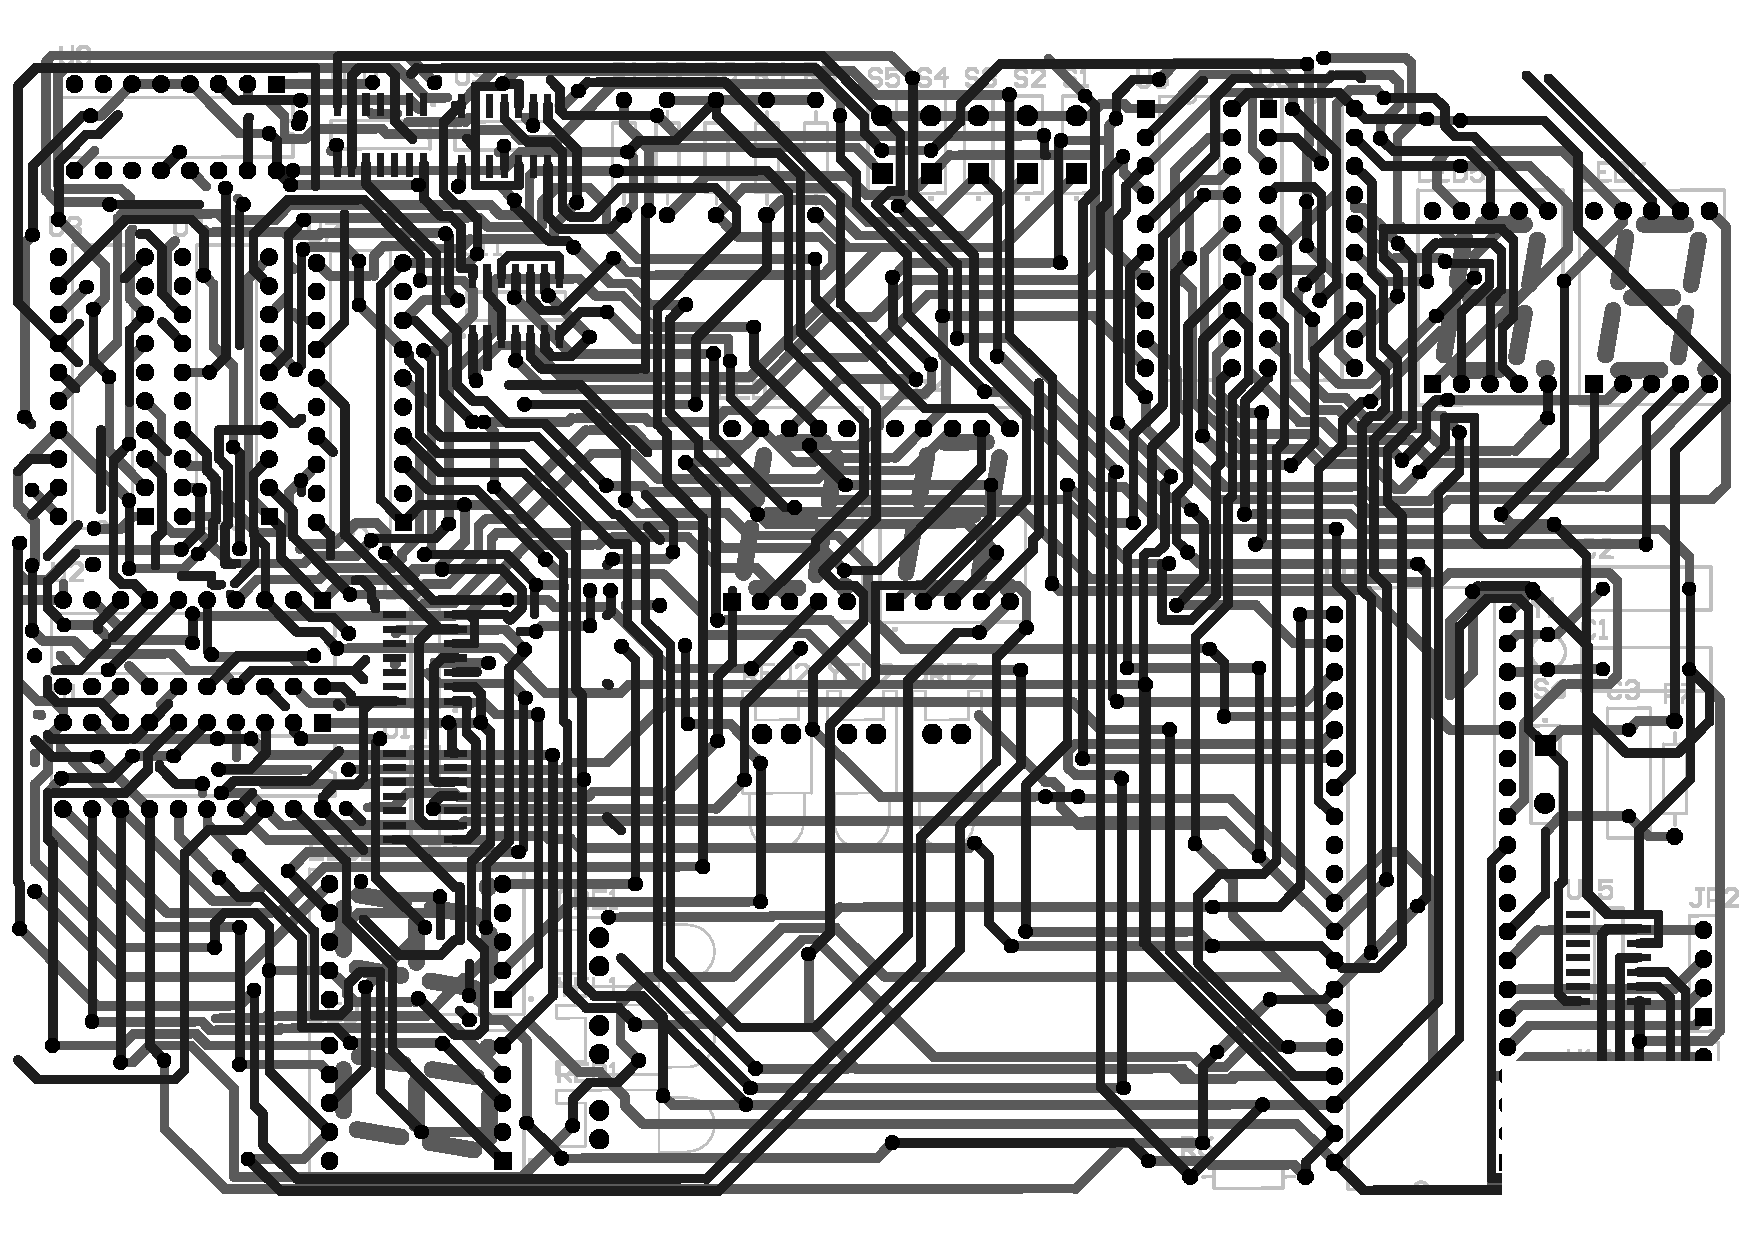
\includegraphics[origin=c, angle= -90,width=0.8\textwidth]{app2/pcb.pdf}
  \bicaption[fig:pcb]{PCB电路图}{PCB版图}{Fig}{PCB Map}
\end{figure}
\label{app:circuit}
\begin{figure}[!bhtb]
  \centering
  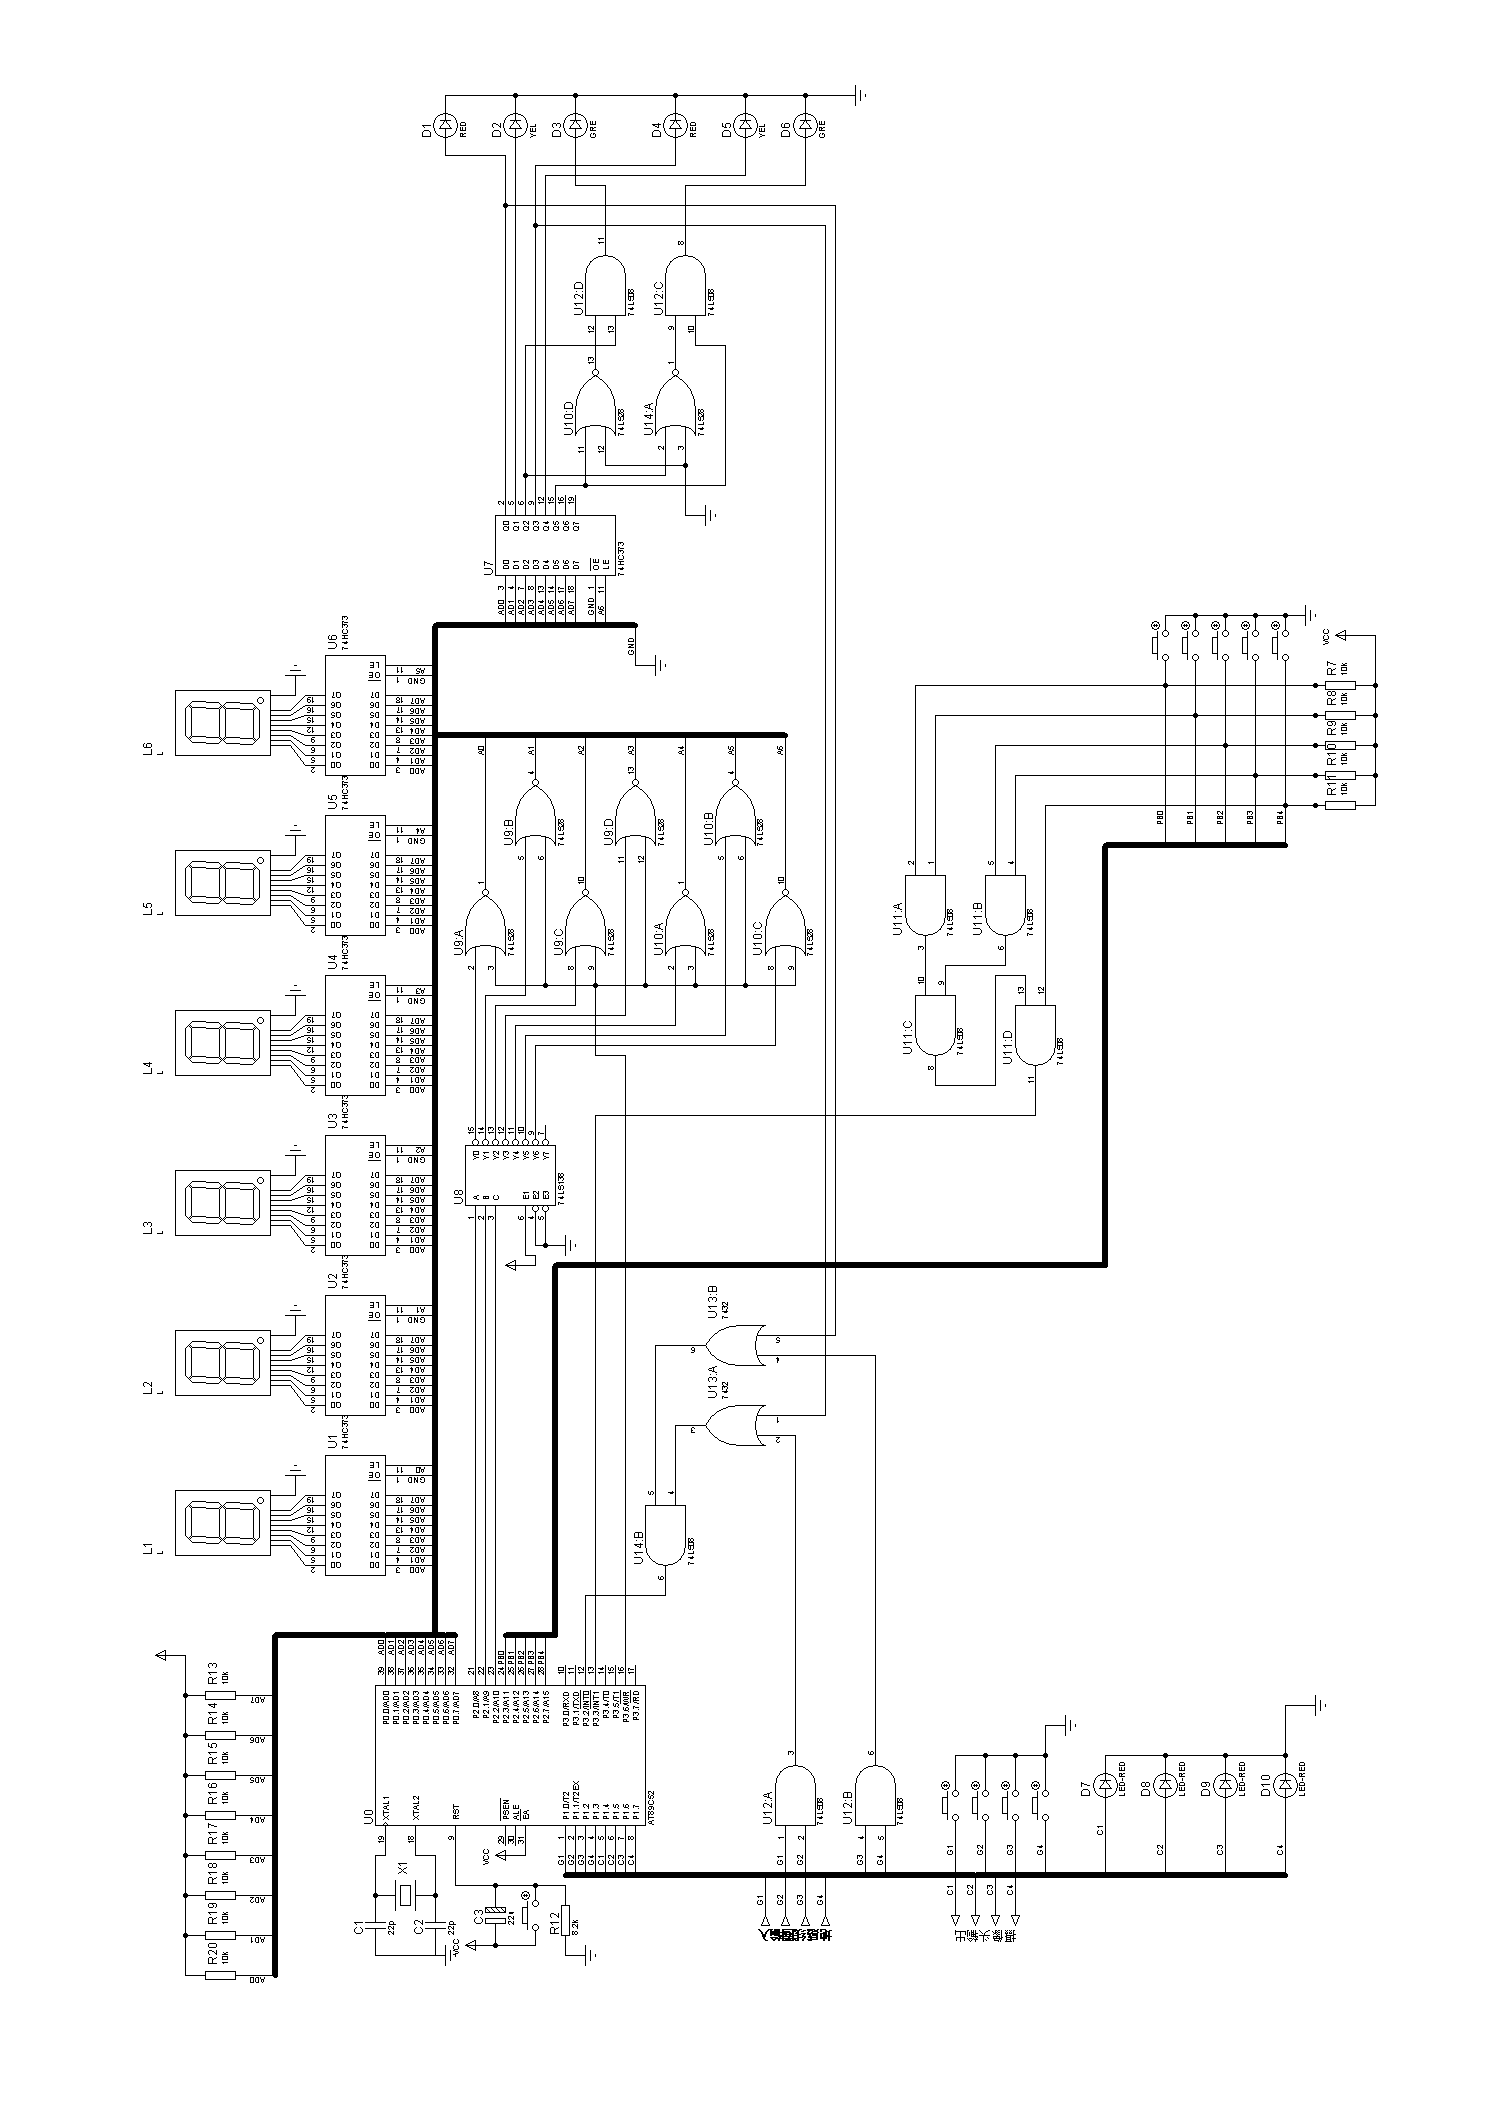
\includegraphics[origin=c, angle= -90,width=0.88\textwidth]{app2/circuitpng.png}
  \bicaption[fig:circuitall]{电路图}{电路图}{Fig}{Circuit Map}
\end{figure}
\begin{figure}[!bhtb]
  \centering
  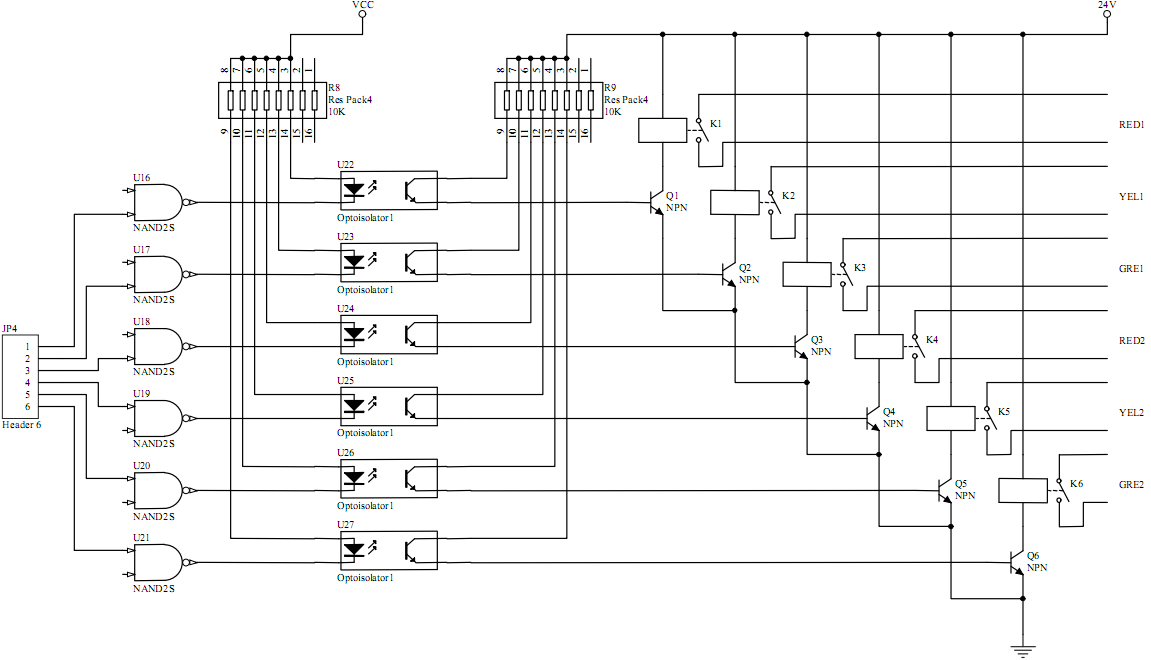
\includegraphics[origin=c, angle= -90,width=0.8\textwidth]{app2/output.png}
  \bicaption[fig:output]{信号灯输出电路}{信号灯输出放大电路}{Fig}{output convert circuit}
\end{figure}


